\documentclass[12pt, a4paper]{article}
% Some fancy symbols
\usepackage{textcomp}
\usepackage{stmaryrd}
\usepackage{cancel}

% Some fancy symbols
\usepackage{textcomp}
\usepackage{stmaryrd}


\usepackage{array}

% Math packages
\usepackage{amsmath,amsthm,amssymb, amsfonts, mathrsfs, dsfont, mathtools}
% \usepackage{mathtext}

\usepackage[bb=boondox]{mathalfa}
\usepackage{bm}

% To conrol figures:
\usepackage{subfig}
\usepackage{adjustbox}
\usepackage{placeins}
\usepackage{rotating}



\usepackage{lipsum}
\usepackage{psvectorian} % Insanely fancy text separators!


% Refs:
\usepackage{url}
\usepackage[backref]{hyperref}

% Fancier tables and lists
\usepackage{booktabs}
\usepackage{enumitem}
% Don't indent paragraphs, leave some space between them
\usepackage{parskip}
% Hide page number when page is empty
\usepackage{emptypage}


\usepackage{multicol}
\usepackage{xcolor}

\usepackage[normalem]{ulem}

% For beautiful code listings:
% \usepackage{minted}
\usepackage{listings}

\usepackage{csquotes} % For citations
\usepackage[framemethod=tikz]{mdframed} % For further information see: http://marcodaniel.github.io/mdframed/

% Plots
\usepackage{pgfplots} 
\pgfplotsset{width=10cm,compat=1.9} 

% Fonts
\usepackage{unicode-math}
% \setmathfont{TeX Gyre Termes Math}

\usepackage{fontspec}
\usepackage{polyglossia}

% Named references to sections in document:
\usepackage{nameref}


% \setmainfont{Times New Roman}
\setdefaultlanguage{russian}

\newfontfamily\cyrillicfont{Kurale}
\setmainfont[Ligatures=TeX]{Kurale}
\setmonofont{Fira Code}

% Common number sets
\newcommand{\sN}{{\mathbb{N}}}
\newcommand{\sZ}{{\mathbb{Z}}}
\newcommand{\sZp}{{\mathbb{Z}^{+}}}
\newcommand{\sQ}{{\mathbb{Q}}}
\newcommand{\sR}{{\mathbb{R}}}
\newcommand{\sRp}{{\mathbb{R^{+}}}}
\newcommand{\sC}{{\mathbb{C}}}
\newcommand{\sB}{{\mathbb{B}}}

% Math operators

\makeatletter
\newcommand\RedeclareMathOperator{%
  \@ifstar{\def\rmo@s{m}\rmo@redeclare}{\def\rmo@s{o}\rmo@redeclare}%
}
% this is taken from \renew@command
\newcommand\rmo@redeclare[2]{%
  \begingroup \escapechar\m@ne\xdef\@gtempa{{\string#1}}\endgroup
  \expandafter\@ifundefined\@gtempa
     {\@latex@error{\noexpand#1undefined}\@ehc}%
     \relax
  \expandafter\rmo@declmathop\rmo@s{#1}{#2}}
% This is just \@declmathop without \@ifdefinable
\newcommand\rmo@declmathop[3]{%
  \DeclareRobustCommand{#2}{\qopname\newmcodes@#1{#3}}%
}
\@onlypreamble\RedeclareMathOperator
\makeatother


% Correction:
\definecolor{correct_color}{HTML}{009900}
\newcommand\correction[2]{\ensuremath{\:}{\color{red}{#1}}\ensuremath{\to }{\color{correct_color}{#2}}\ensuremath{\:}}
\newcommand\inGreen[1]{{\color{correct_color}{#1}}}

% Roman numbers && fancy symbs:
\newcommand{\RNumb}[1]{{\uppercase\expandafter{\romannumeral #1\relax}}}
\newcommand\textbb[1]{{$\mathbb{#1}$}}



% MD framed environments:
\mdfsetup{skipabove=1em,skipbelow=0em}

% \mdfdefinestyle{definition}{%
%     linewidth=2pt,%
%     frametitlebackgroundcolor=white,
%     % innertopmargin=\topskip,
% }

\theoremstyle{definition}
\newmdtheoremenv[nobreak=true]{definition}{Определение}
\newmdtheoremenv[nobreak=true]{theorem}{Теорема}
\newmdtheoremenv[nobreak=true]{lemma}{Лемма}
\newmdtheoremenv[nobreak=true]{problem}{Задача}
\newmdtheoremenv[nobreak=true]{property}{Свойство}
\newmdtheoremenv[nobreak=true]{statement}{Утверждение}
\newmdtheoremenv[nobreak=true]{corollary}{Следствие}
\newtheorem*{note}{Замечание}
\newtheorem*{example}{Пример}

% To mark logical parts
\newcommand{\existence}{{\circled{$\exists$}}}
\newcommand{\uniqueness}{{\circled{$\hspace{0.5px}!$}}}
\newcommand{\rightimp}{{\circled{$\Rightarrow$}}}
\newcommand{\leftimp}{{\circled{$\Leftarrow$}}}


% Useful symbols:
\renewcommand{\qed}{\ensuremath{\blacksquare}}
\renewcommand{\vec}[1]{\overrightarrow{#1}}
\newcommand{\eqdef}{\overset{\mathrm{def}}{=\joinrel=}}
\newcommand{\isdef}{\overset{\mathrm{def}}{\Longleftrightarrow}}
\newcommand{\inductdots}{\ensuremath{\overset{induction}{\cdots}}}

% Matrix's determinant
\newenvironment{detmatrix}
{
  \left|\begin{matrix}
}{
  \end{matrix}\right|
}

\newenvironment{complex}
{
  \left[\begin{gathered}
}{
  \end{gathered}\right.
}


\newcommand{\nl}{$~$\\}

\newcommand{\tit}{\maketitle\newpage}
\newcommand{\tittoc}{\tit\tableofcontents\newpage}


\newcommand{\vova}{  
    Латыпов Владимир (конспектор)\\
    {\small \texttt{t.me/donRumata03}, \texttt{github.com/donRumata03}, \texttt{donrumata03@gmail.com}}
}


\usepackage{tikz}
\newcommand{\circled}[1]{\tikz[baseline=(char.base)]{
            \node[shape=circle,draw,inner sep=2pt] (char) {#1};}}

\newcommand{\contradiction}{\circled{!!!}}

% Make especially big math:

\makeatletter
\newcommand{\biggg}{\bBigg@\thr@@}
\newcommand{\Biggg}{\bBigg@{4.5}}
\def\bigggl{\mathopen\biggg}
\def\bigggm{\mathrel\biggg}
\def\bigggr{\mathclose\biggg}
\def\Bigggl{\mathopen\Biggg}
\def\Bigggm{\mathrel\Biggg}
\def\Bigggr{\mathclose\Biggg}
\makeatother


% Texts dividers:

\newcommand{\ornamentleft}{%
    \psvectorian[width=2em]{2}%
}
\newcommand{\ornamentright}{%
    \psvectorian[width=2em,mirror]{2}%
}
\newcommand{\ornamentbreak}{%
    \begin{center}
    \ornamentleft\quad\ornamentright
    \end{center}%
}
\newcommand{\ornamentheader}[1]{%
    \begin{center}
    \ornamentleft
    \quad{\large\emph{#1}}\quad % style as desired
    \ornamentright
    \end{center}%
}


% Math operators

\DeclareMathOperator{\sgn}{sgn}
\DeclareMathOperator{\id}{id}
\DeclareMathOperator{\rg}{rg}
\DeclareMathOperator{\determinant}{det}

\DeclareMathOperator{\Aut}{Aut}

\DeclareMathOperator{\Sim}{Sim}
\DeclareMathOperator{\Alt}{Alt}



\DeclareMathOperator{\Int}{Int}
\DeclareMathOperator{\Cl}{Cl}
\DeclareMathOperator{\Ext}{Ext}
\DeclareMathOperator{\Fr}{Fr}


\RedeclareMathOperator{\Re}{Re}
\RedeclareMathOperator{\Im}{Im}


\DeclareMathOperator{\Img}{Im}
\DeclareMathOperator{\Ker}{Ker}
\DeclareMathOperator{\Lin}{Lin}
\DeclareMathOperator{\Span}{span}

\DeclareMathOperator{\tr}{tr}
\DeclareMathOperator{\conj}{conj}
\DeclareMathOperator{\diag}{diag}

\expandafter\let\expandafter\originald\csname\encodingdefault\string\d\endcsname
\DeclareRobustCommand*\d
  {\ifmmode\mathop{}\!\mathrm{d}\else\expandafter\originald\fi}

\newcommand\restr[2]{{% we make the whole thing an ordinary symbol
  \left.\kern-\nulldelimiterspace % automatically resize the bar with \right
  #1 % the function
  \vphantom{\big|} % pretend it's a little taller at normal size
  \right|_{#2} % this is the delimiter
  }}

\newcommand{\splitdoc}{\noindent\makebox[\linewidth]{\rule{\paperwidth}{0.4pt}}}

% \newcommand{\hm}[1]{#1\nobreak\discretionary{}{\hbox{\ensuremath{#1}}}{}}


\usepackage{geometry}
\geometry{
    a4paper,
    left=13mm,
    right=13mm,
    top=15mm,
    bottom=15mm
}

\graphicspath{{res/}}


\title{Теорвер. Домашнее задание №3 \\ \large Случайные величины} 

\author{
  Латыпов Владимир
}

\date{\today}



\begin{document}
\maketitle


\section{Каким идти на экзамен}

У первого: $\frac{n}{N}$.

У второго: 

\begin{equation}
  p_{\text{first is lucky}} \cdot \frac{n - 1}{N - 1} + p_{\text{first isn't lucky}} \cdot \frac{n}{N - 1} =
  \frac{n}{N} \cdot \frac{n - 1}{N - 1} + \frac{N - n}{N} \cdot \frac{n}{N - 1} = \frac{n}{N}
\end{equation}

Аналогично — у третьего. Странно, если было бы иначе, ведь каждая перестановка равновероятна (обсуждали ещё на дискретке),
а количество перестановок с хорошим билетом на месте: $n \cdot (N - 1)!$ из всех $N (N - 1)!$.

Note: частный случай следующей задачи для $k = -1$…

\section{Случайное копирование}

Исходное $\Omega$ — битовые векторы выборов (aka ветки в полном бинарном дереве выбора), у каждого своя вероятность, однако суммарная вероятность $= 1$.

Нужно найти суммарную вероятность тех веток длины $s$, в которых последний шаг равен нулю (белый шар).

Однако заметим, что, если знать матожидание \textit{процента белых шаров \textbf{после}} $s - 1$\textit{-го шага} (назовём этот процент — случайную величину), то это и будет искомая вероятность.

\begin{equation}
  E[W_{s - 1}] = \sum_{\omega \in \Omega_{s - 1}} W_{s - 1}(\omega) p(\omega)
\end{equation}


\begin{equation}
  p(\text{s th is white}) = \sum_{\omega \in \Omega_{s}} [\omega_{n - 1} = \text{White}] p(\omega)  = \sum_{\omega' \in \Omega_{s - 1}} 1 \cdot W_{s - 1}(\omega') p(\omega') + 0 \cdot p(\omega') (1 - W_{s - 1}(\omega'))
\end{equation}

Попробуем выразить $E[W_{s}]$, зная $E[W_{s - 1}]$.

По формуле полного матожидания (разделим все исходы на два события: выпал в $s$-ый раз белый шар или нет):

\begin{multline}
  E[W_{s}] = \sum_{\omega \in \Omega_{s}} W_{s}(\omega) p(\omega) = \\
  \sum_{\omega \in \Omega_{s}} \frac{M(\omega)}{N(\omega) + M(\omega)} p(\omega) = \\
  \sum_{\omega \in \Omega_{s - 1}} \frac{M(\omega \#\# 0)}{N(\omega \#\# 0) + M(\omega \#\# 0)} p(\omega \#\# 0) + \frac{M(\omega \#\# 1)}{N(\omega \#\# 1) + M(\omega \#\# 1)} p(\omega \#\# 1) = \\
  \sum_{\omega \in \Omega_{s - 1}} \frac{M(\omega) + k}{N(\omega) + M(\omega) + k} p(\omega) \frac{M(\omega)}{N(\omega) + M(\omega)}
   + \frac{M(\omega) + k}{N(\omega) + M(\omega) + k} p(\omega) \frac{N(\omega)}{N(\omega) + M(\omega)} = \\
   \sum_{\omega \in \Omega_{s - 1}} \frac{N(\omega)}{N(\omega) + M(\omega)} p(\omega) = \sum_{\omega \in \Omega_{s - 1}} W_{s - 1}(\omega) p(\omega) = E[W_{s - 1}]
\end{multline}

В предпредпоследнем переходе мы воспользовались \url{https://www.wolframalpha.com/input?i=%28m+%2B+k%29+%2F+%28n+%2B+m+%2B+k%29+m%2F%28n+%2B+m%29+%2B+%28m%29+%2F+%28n+%2B+m+%2B+k%29+n%2F%28n+%2B+m%29}.


\begin{equation}
  p(\text{s th is white}) E[W_{s} | \text{s th is white}] + (1 - p(\text{s th is white})) E[W_{s} | \text{s th isn't white}] = \\
  E[W_{s - 1}] E[W_{s} | \text{s th is white}] + (1 - E[W_{s - 1}]) E[W_{s} | \text{s th isn't white}] = TODO \\
  \left(\sum_{\omega \in \Omega_{s - 1}} W_{s - 1}(\omega) p(\omega)\right) = E[W_{s - 1}]
\end{equation}

\section{Случайный диодный мост с замыканием}

Убьём двух зайцев, разделив $\Omega$ на события «$E$ открыто» ($E$) и «$E$ закрыто» ($\overline{E}$).

$S$ — success.

\begin{equation}
  P(S | E) = P(A \cup C) \cdot P(B \cup D) = (1 - P(\overline{A}\overline{C}))^2 = (1 - (1 - p)^2)^2 = 4 p^2 - 4 p^3 + p^4
\end{equation}

\begin{equation}
  P(S | \overline{E}) = P(AB \cup CD) = P(AB) + P(CD) - P(ABCD) = 2p^2 - p^4
\end{equation}

\begin{gather}
  P(S) = P(E) P(S | E) + P(\overline{E}) P(S | \overline{E}) = p (4 p^2 - 4 p^3 + p^4) + (1 - p)(2p^2 - p^4) = 2 p^5 - 5 p^4 + 2 p^3 + 2 p^2 \\
  P(E | S) = \frac{P(E) P(S | E)}{P(S)} = \frac{p (4 p^2 - 4 p^3 + p^4)}{2 p^5 - 5 p^4 + 2 p^3 + 2 p^2}
\end{gather}



\section{Диффур потребления}

\subsection{Для случая одного механизма}

$p = P_1, (1 - p) = P_0$.

Записав условие задачи, получим определение дифференцируемости:

\begin{equation}
  p(t + \Delta t) = p(t) - p(t) (\alpha \Delta t + o(\Delta t)) + 
  (1 - p(t)) (\beta \Delta t + o(\Delta t))
\end{equation}

То есть диффур: $p' = -\alpha p + \beta(1 - p) = (-\alpha - \beta) p + \beta$


\subsection{Общий случай}

Случаи, когда мутировало больше одного механизма случаются с вероятностью $o(\Delta t)$,
их конечное количество, так что и сумма такова.

\begin{multline}
  P_r(t + \Delta t) = P_r(t) + \sum_{k = 0}^n P_k(t) p_{kr} - P_r(t) \left(\alpha \binom{r}{1} \Delta t + o(\Delta t)\right) \\
  = P_r(t) - P_r(t) \alpha r \Delta t + P_{r - 1}(t) \beta (n - r + 1) \Delta t + P_{r + 1}(t) \alpha (n - r + 1) \Delta t + o(\Delta t) 
\end{multline}

(Полагаем $P_i(t) = 0$ для $i \notin [0, n]$)

Получаем систему диффуров:

\begin{equation}
  P'_r(t) = P_r(t)((n - r)\beta - r \alpha) \alpha r + P_{r - 1}(t) \beta (n - r + 1) + P_{r + 1}(t) \alpha (n - r + 1) \quad \forall r \in [0..n]
\end{equation}

ЛОС с разреженной матрицей




\section{Независимость случайных величин}

Интуитивно: какие же они независимые, они чётко выражаются одна через другую,
то есть одна даёт полную информацию о другой.

Проверим определение: $f_{\xi, \nu}(x, y) = f_\xi(x)f_\nu(y)$ (опять интуитивно: не-ноль на пути не представим в виде тензроного произведения).

Но это уже гарантированно неправда: например, для $x = \frac{1}{2}, y = \cos(1)$:
$f_{\xi, \nu}(x, y) = 0$, ведь эти условия несовместны в окрестности.

С другой стороны, оба $f_\xi(x), f_\nu(y)$ не нули, так как в окрестности 
функции дифференцируемы, производная обратной функции не ноль, функция плотности очень даже не ноль.

\begin{figure}[h!]
  \centering
  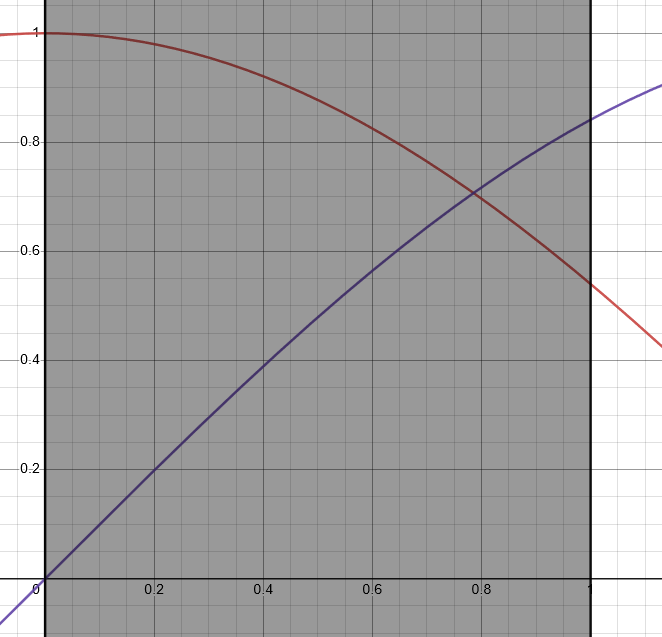
\includegraphics[width=0.5\paperwidth]{res/5.png}
  \caption{Случайные величины}
  \label{fig:counterexample}
\end{figure}
\FloatBarrier


В силу возрастания синуса на $\Omega$:

\begin{equation}
  P(a \leqslant sin(\omega) \leqslant b) = P(\arcsin(a) \leqslant \omega \leqslant \arcsin(b))
\end{equation}


\section{Парадокс Монти Холла}

На самом деле, он должен был понять про апостериорные вероятности
помилования для трёх заключённых следующее: у него — $1/3$, у названного — $0$,
у не названного $2/3$.

В терминах шоу — вопрошающему стоит сменить тело, а не оставаться в своём.

Если формально:

Назовём их $R_1$ (названный), $R_2$ (оставшийся), $R_3$ (он).

$\Omega = {(R_i, S_j)}$


\begin{equation}
  p(R_2 | S_1) = \frac{p(R_2 S_1)}{p(S_1)} = \frac{p(R_2) p(S_1 | R_2)}{p(R_2) p(S_1 | R_2) + p(R_3) p(S_1 | R_3)} = 
  \frac{1/3 \cdot 1}{1/3 \cdot 1 + 1/3 \cdot 1/2} = \frac{2}{3}
\end{equation}

В чём не прав заключённый? Почему он решил, что $1/2$?
Если есть несколько событий, это ещё не значит, что они равновероятны.

Информации о себе он действительно не получил,
так как в любом случае услышал бы неизвестную фамилию.

А вот об оставшемся человеке — информации добавилось: 
если бы он был помилован, вероятность, что стражник об этом скажет — $100\%$,
а если помилован был автор, то лишь $50\%$.
Вероятность помилования от обоих незнакомцев распределилась к нему. 


\paragraph{Доп. вопрос} Когда $\xi$ и $\xi^2$ независимы?

\begin{equation}\label{eq:indep}
  p_{\xi, \xi^2}(x, y) = p_\xi(x)p_{\xi^2}(y)
\end{equation}

Для отрицательных $y$ это тривиально. Рассмотрим, например, положительные $\xi$.
Упорядочим по возрастанию и занумеруем в этом порядке $\xi(\Omega) = x_1, … x_n$.

Тогда $\xi^2(\Omega) = x_1^2, … x_n^2$.

Совместный график будет выглядеть как парабола на прямоугольничке.

\begin{equation}
  p_{\xi, \xi^2}(x, y) = \begin{cases}
    p_\xi(x) & x^2 = y \\
    0 & \text{otherwise}
  \end{cases}
\end{equation}

Если найдутся два разных значения $\xi^2$: $y_1 = x_1^2, y_2 = x_2^2$,
принимаемые с ненулевой вероятностью (на множестве ненулевой меры Лебега-Стилтьеса)
то найдутся и два различных значения $\xi$ с тем же свойством: $x_1, x_2$.

Тогда равенство \ref{eq:indep} нарёшается при $x = x_1, y = y_2$.

Иначе (если все значения, принимаемые $\xi$ с положительной вероятностью, одинаковы) $\xi^2$
независима с чем угодно.


\section{Выпускной}

Элементарные исходы: случайные векторы выборов — для каждого студента — то, куда он пошёл.
Вероятность каждого: $\frac{1}{n^k}$.

По линейности матожидания достаточно
посчитать матожидание количество пролетевших студентов в одном заведении:

\begin{equation}
  E[N_{\mathrm{fail}}] = E\left[\sum_{i = 1}^n \mathrm{failed}_i\right] = \sum_{s = 1}^n E[\mathrm{failed}_i] = n E[\mathrm{failed}_i]
\end{equation}

\begin{equation}
  P([N_i = x]) = [\text{vec with N(i) = x}] = \frac{\binom{k}{x} \cdot (n - 1)^{k - x}}{n^k}
\end{equation}

\begin{multline}
  E[\mathrm{failed}_i] = E\left[\begin{cases}
    N_i - r & N_i \geqslant r, \\
    0 & \text{otherwise}
  \end{cases}\right] = -r + \sum_{x = r}^{k} x P([N_i = x]) = -r + \sum_{x = r}^{k} x P([N_i = x]) = \\
  -r + \frac{1}{n^r}\sum_{x = r}^{k} x \binom{k}{x} \cdot (n - 1)^{k - x}
\end{multline}

\begin{equation}
  E[N_{\mathrm{fail}}] = E\left[\sum_{i = 1}^n \mathrm{failed}_i\right] = \sum_{s = 1}^n E[\mathrm{failed}_i] = n E[\mathrm{failed}_i] = 
  -rn + \frac{1}{n^{r - 1}}\sum_{x = r}^{k} x \binom{k}{x} \cdot (n - 1)^{k - x}
\end{equation}

Рассмотрим студента и заведение, которое он выбрал $p_s$ — вероятность, что туда

\section{Оптимизация}

\begin{equation}
  \begin{cases}
    3 (p - p^2) \leqslant 1 \\
    2p^2 \leqslant p
  \end{cases}
\end{equation}

$1/2$ — достигается при $\{a, b, c, d\}; P(x) = 1/4; A = \{a, b\}, B = \{b, c\}, D = \{c, a\}$


\section{Три вещи несовместные — как ты да я}

\begin{equation}
  0 = P(AB) \neq P(A) P(B) > 0
\end{equation}

Чтобы $AB$ и $A \cup B$ были независимы:

\begin{equation}
  p(AB \cap (A \cup B)) = p(ABA \cup ABB) = p(AB) = [\text{independence}] = p(AB)p(A \cup B)
\end{equation}

То есть события должны быть либо несовместными, либо вместе составлять всё пространство.

\end{document}
